\documentclass[handout]{beamer}
\usepackage[utf8]{inputenc}
\usepackage{amsmath, pdfpages, pdflscape, lscape, color, listings, hyperref, amssymb, graphicx,textcomp,varioref, afterpage, subcaption, float, bm, tikz, multicol}

\global
\newcommand{\Fig}[1]{Figure \ref{#1}}
\newcommand{\fig}[1]{figure \ref{#1}}
\newcommand{\tab}[1]{table \ref{#1}}
\newcommand{\eq}[1]{equation \ref{#1}}
\newcommand{\Eq}[1]{Equation \ref{#1}}
\newcommand{\alg}[1]{algorithm \ref{#1}}
\newcommand{\Alg}[1]{Algorithm \ref{#1}}
\newcommand{\chp}[1]{chapter  \ref{#1}}
\newcommand{\Chp}[1]{Chapter  \ref{#1}}
\newcommand{\e}[1]{\cdot 10^{#1}}
\newcommand{\h}{\hbar}
\newcommand{\der}[2]{\frac{\partial #1}{\partial #2}}
\newcommand{\dder}[2]{\frac{\partial^2 #1}{\partial #2^2}}
\newcommand{\p}{\boldsymbol{P}}
\newcommand{\q}{\boldsymbol{q}}
\newcommand{\norm}[1]{\left\lVert#1\right\rVert_{\!Q}}
\newcommand{\inner}[1]{\left\langle #1\right\rangle_{\!Q}}
\newcommand{\coef}[2]{\frac{\langle #1,#2\rangle_{\!Q}}{\norm{#2}^2}}


\DeclareMathOperator*{\argmin}{argmin}
\DeclareMathOperator*{\argmax}{argmax}

\newcommand{\E}[1]{\mbox{E}\!\left(#1\right)}
\newcommand{\Var}[1]{\mbox{Var}\!\left(#1\right)}
\newcommand{\Cov}[1]{\mbox{Cov}\!\left(#1\right)}

\newenvironment{test}[1]
{
 \usebackgroundtemplate{}
 \color{gray!30!black}
   \begin{tikzpicture}[remember picture, overlay]
     \node[anchor = center, opacity=.25] (image) at (current page.center) {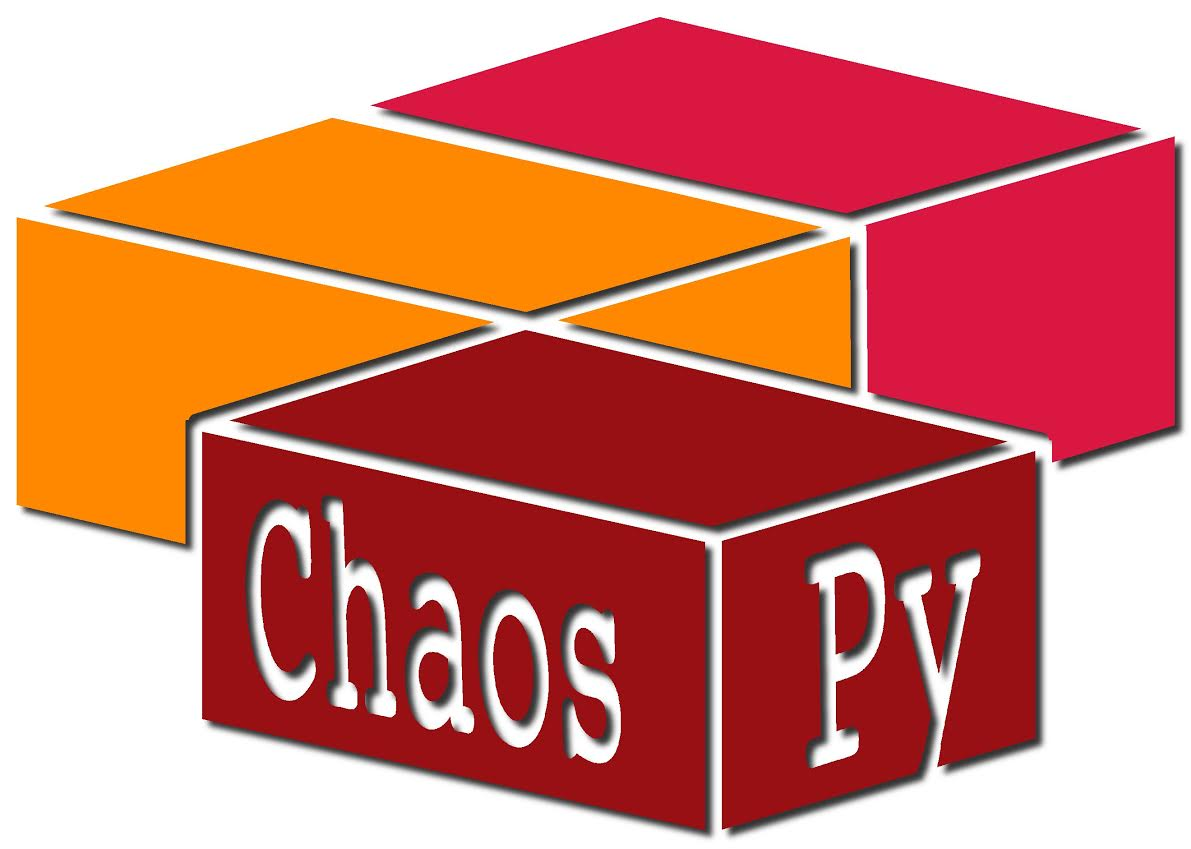
\includegraphics[scale=0.25]{chaospy_logo.jpg}};
   \end{tikzpicture}
 \begin{frame}[fragile,enviroment=chaospy]

}
{
 \end{frame}
}


 \lstset{
escapeinside={||},
basicstyle=\ttfamily\footnotesize,
columns=fixed
}

\newenvironment{chaospy}[1]
{\color{gray!30!black}
     \color{gray!30!black}
     \usebackgroundtemplate{
   \begin{tikzpicture}[remember picture, overlay]
     \node[anchor = center, opacity=.25] (image) at (current page.center) {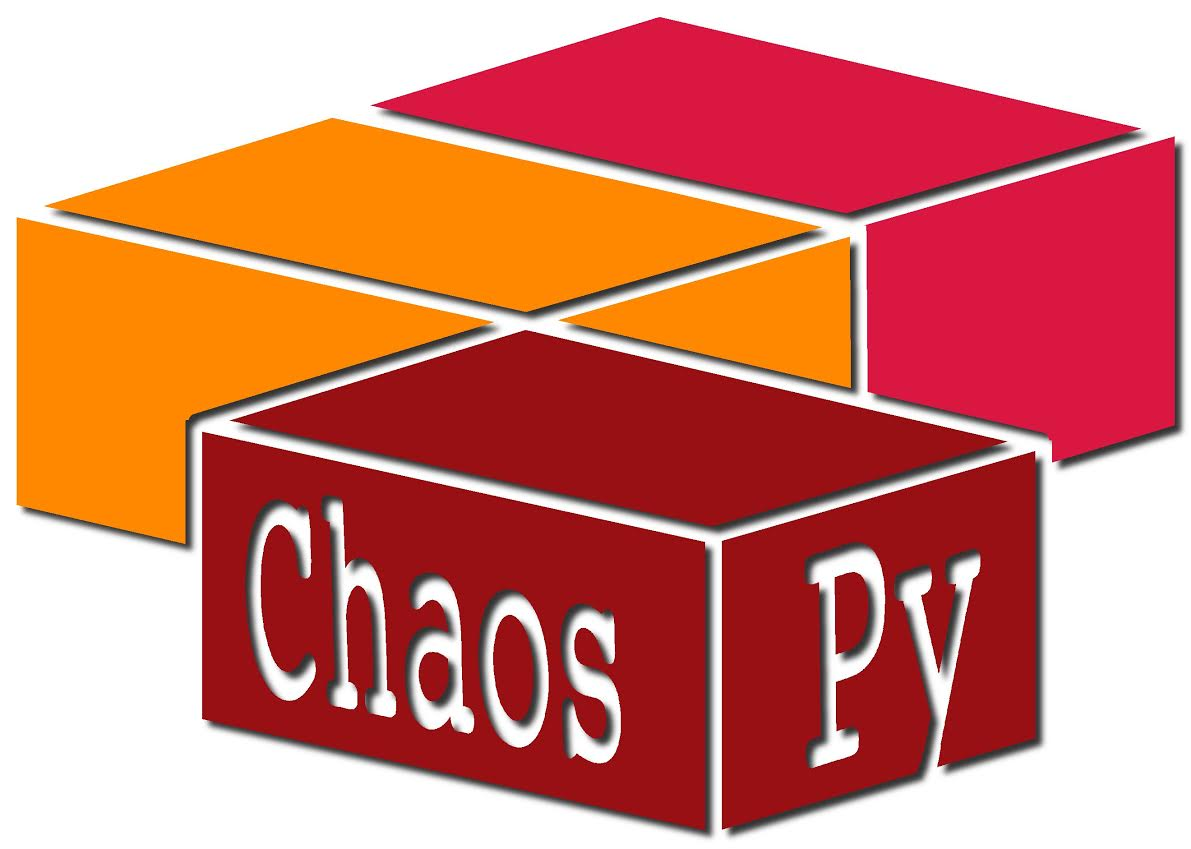
\includegraphics[scale=0.25]{chaospy_logo.jpg}};
   \end{tikzpicture}}
     \begin{frame}[fragile,environment=chaospy]
    \frametitle{{#1}}}
{\end{frame}}


\definecolor{keywords}{RGB}{255,0,90}
\definecolor{comments}{RGB}{0,0,113}
\definecolor{red}{RGB}{160,0,0}
\definecolor{green}{RGB}{0,150,0}

\usetheme{kalkulo}

\graphicspath{{./figures/}}


\title{Polynomial chaos expansions part 4: Generalized polynomial
chaos}
\author{Jonathan Feinberg and Simen Tennøe}


\begin{document}



\begin{frame}
  \maketitle
\end{frame}


\begin{frame}
 \frametitle{Some random variables are dependent}
 \begin{figure}
 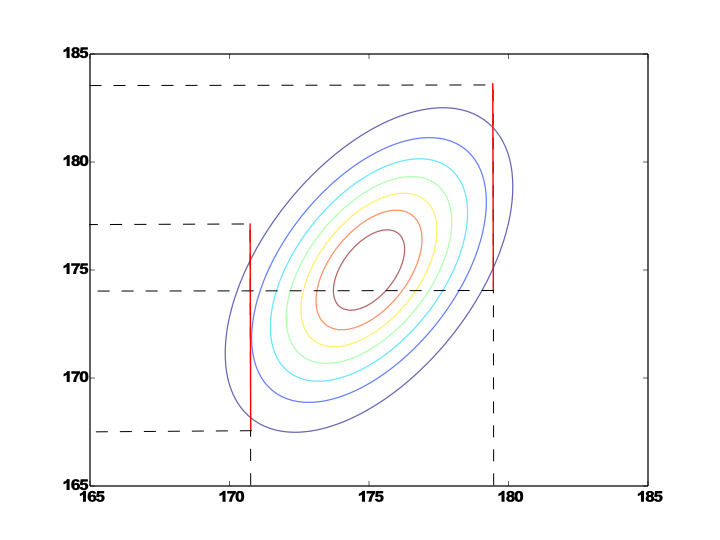
\includegraphics[width = 0.9\textwidth]{dependent.png}
 \end{figure}

 \end{frame}


 \begin{chaospy}{Repetition of our model problem with two independent variables $I$ and $a$}
     \scriptsize
 \begin{lstlisting}[language=python]
def u(x,a, I):
  return I*np.exp(-a*x)
|\pause|
dist_a = cp.Uniform(0, 0.1)
dist_I = cp.Uniform(8, 10)
dist = cp.J(dist_a, dist_I)
|\pause|
P = cp.orth_ttr(2, dist)
|\pause|
nodes, weights = \
    cp.generate_quadrature(3, dist, rule="G")
|\pause|
x = np.linspace(0, 10, 100)
samples_u = [u(x, *node) for node in nodes.T]
|\pause|
u_hat = cp.fit_quadrature(P, nodes, weights, samples_u)
 \end{lstlisting}
\end{chaospy}


\begin{frame}
 \frametitle{Dependent variables break the orthogonality property of polynomials!}
 \scriptsize
 \[  P_{\mathfrak i} = P_{i_1}^{(1)}P_{i_2}^{(2)}\cdots P_{i_D}^{(D)} \qquad \mathfrak i = (i_1,i_2,...,i_D)\]
 \pause
 \begin{align*}
     \inner{ P_\mathfrak{i},P_\mathfrak{j}} &= E(P_\mathfrak{i},P_\mathfrak{j})\\
  \onslide<3-> {&=\E{P_{i_1}^{(1)}\cdots P_{i_D}^{(D)}P_{j_1}^{(1)}\cdots P_{j_D}^{(D)}}}\\
  \onslide<4-> {&=\E{P_{i_1}^{(1)}P_{j_1}^{(1)}}\cdots \E{P_{i_D}^{(D)}P_{j_D}^{(D)}}}\\
  \onslide<5-> {&=\dots}\\
  \onslide<5-> {&=\norm{P_{\mathfrak{i}}^{(1)}}\delta_{\mathfrak{i}\mathfrak{j}}}
 \end{align*}
 \onslide<6->
\begin{alert}{But the problem is:}
\[\E{uv} \neq \E{u}\E{v} \qquad \text{when $u$ and $v$ are
stochastically dependent}\]
 \end{alert}

\end{frame}


\begin{frame}{Transformations manipulates probability distributions}
\begin{figure}
 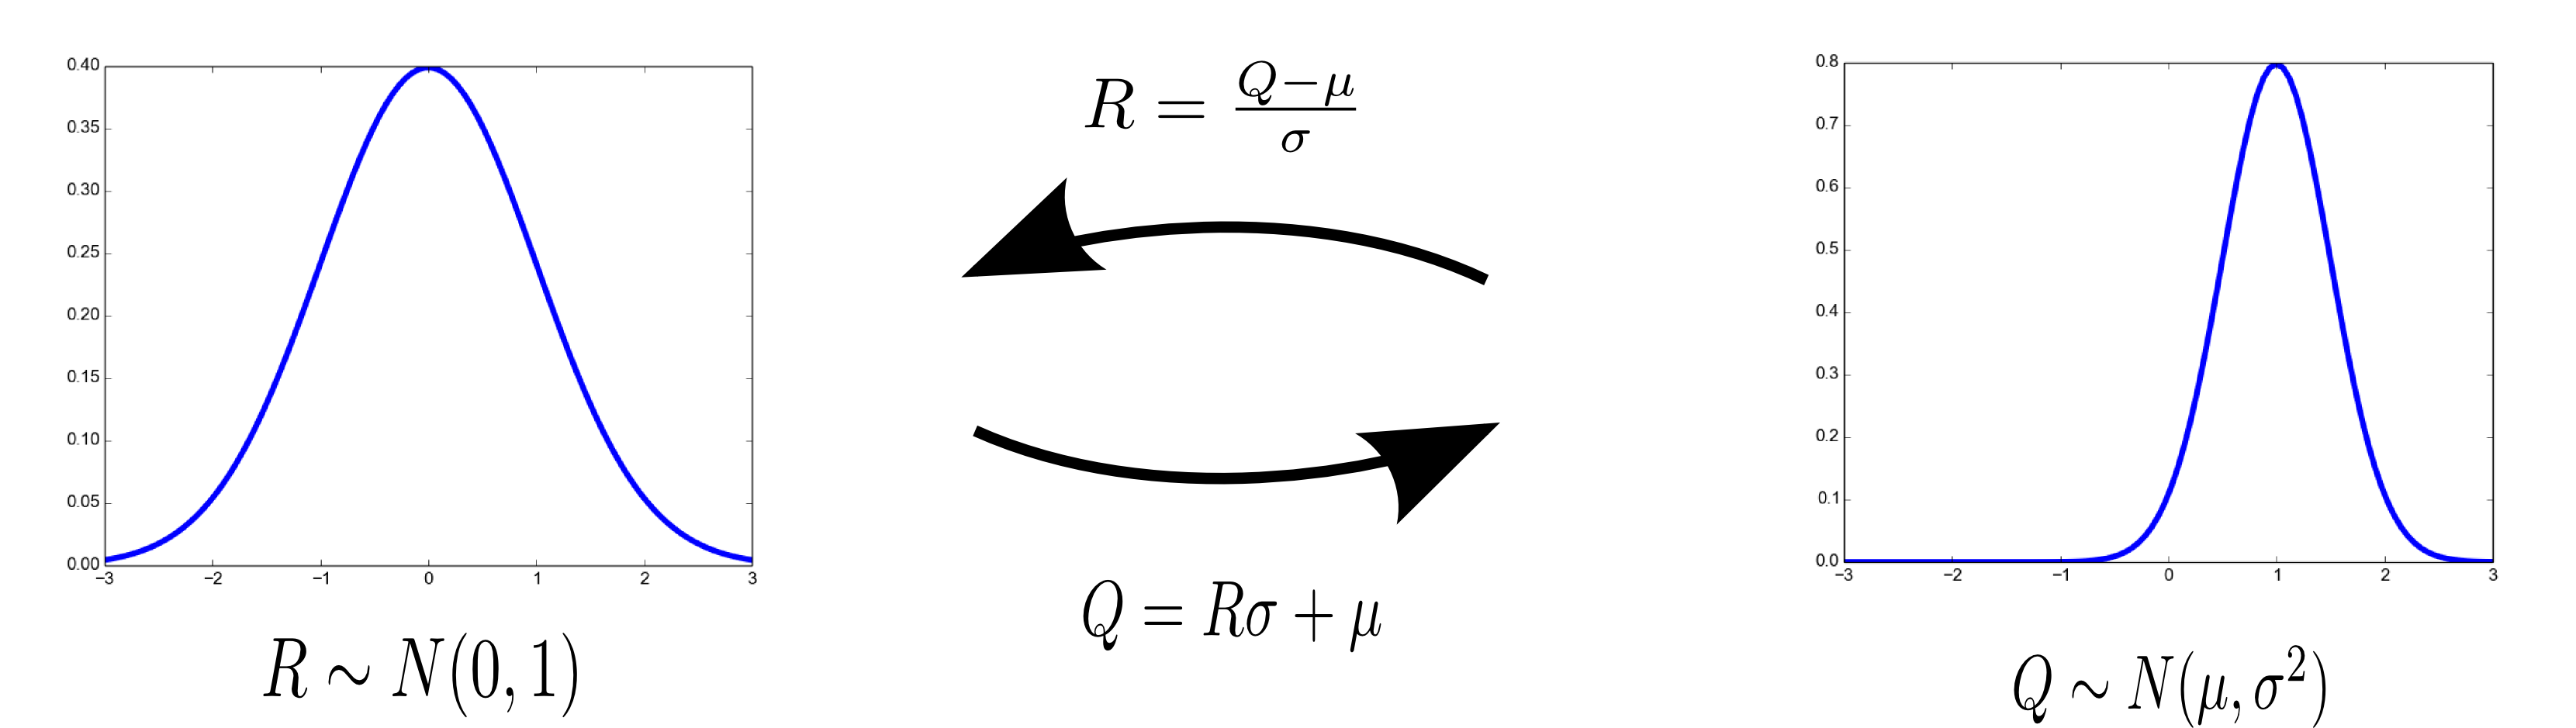
\includegraphics[width=\textwidth]{trans2.png}
\end{figure}
\end{frame}


\begin{frame}{Transformation for multivariate distributions}{}
\begin{figure}
 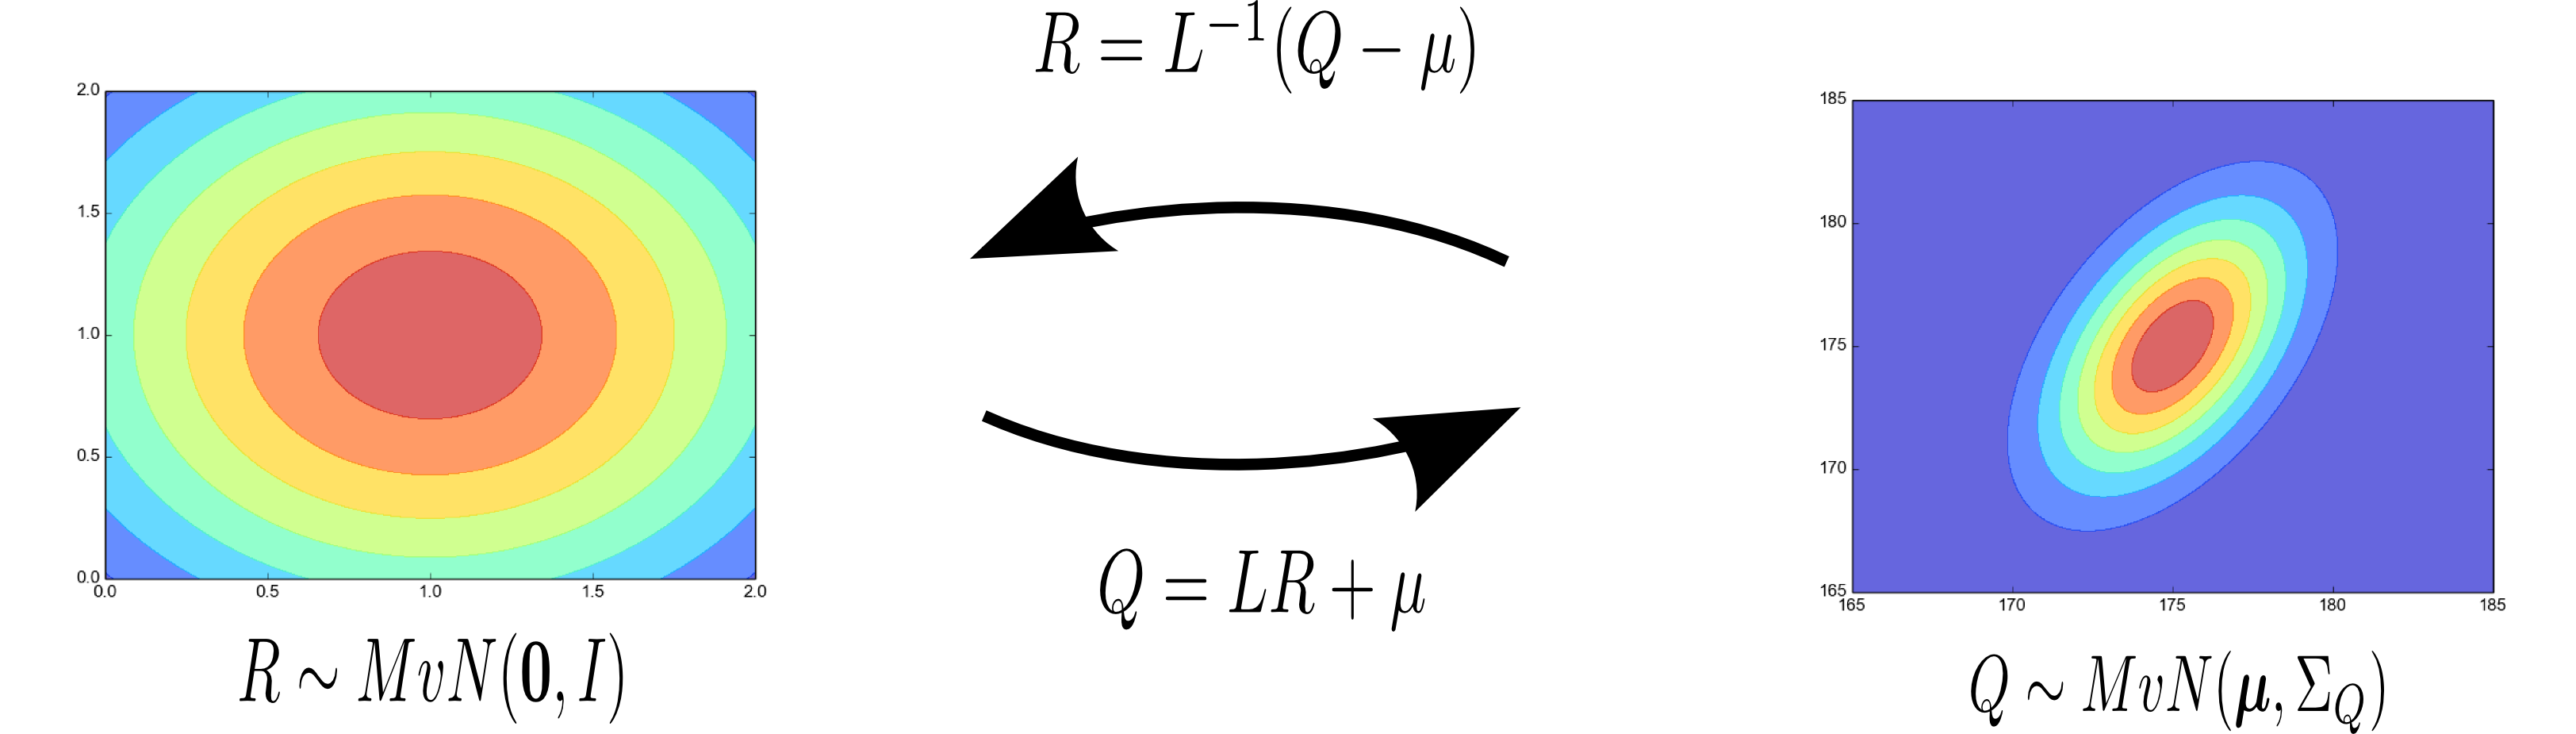
\includegraphics[width=\textwidth]{trans1.png}
\end{figure}
    \begin{flushright}
        $\Sigma_Q = L^TL$
    \end{flushright}
    \scriptsize
\pause
    \begin{align*}
        \bm\mu_Q &=
        \begin{pmatrix}
            0 \\ 0
        \end{pmatrix} &
        \Sigma_Q &=
        \begin{pmatrix}
            1 & \rho \\ \rho & 1
        \end{pmatrix} &
        \bm\mu_R &=
        \begin{pmatrix}
            0 \\ 0
        \end{pmatrix} &
        \Sigma_R &=
        \begin{pmatrix}
            1 & 0 \\ 0 & 1
        \end{pmatrix}
    \end{align*}
    \pause
    \normalsize
    \begin{align*}
        Q_1(R_1, R_2) &= R_1 &
        Q_2(R_1, R_2) &= \rho R_2 + \sqrt{1-\rho^2} R_1
    \end{align*}
\end{frame}

\begin{frame}{Transformations can be used to model dependent
    variables effectively as a parameterization of independent
    variables}{}
    \begin{align*}
        \hat u_M(x; q)
        \onslide<2->{= \hat u_M(x; T(r))}
        \onslide<3->{= \sum_{n=0}^N c_n(x) P_n(r)}
    \end{align*}
\end{frame}

\begin{chaospy}{Code for dependent normal variables}
 \scriptsize
 \begin{lstlisting}[language=Python]
x = np.linspace(0, 1, 100)
def u(x, a, I):
  return I*np.exp(-a*x)

C = [[2,1],[1,2]]
mu = [0.5,0.5]
|\pause|
dist_R = cp.J(cp.Normal(), cp.Normal())|\pause|
P = cp.orth_ttr(M, dist_R)|\pause|
L =  np.linalg.cholesky(C)      # C = np.dot(L.T, L) |\pause|
def T(r):
    return np.dot(L,r) + mu
|\pause|
nodes_R = dist_R.sample(2*len(P), "M")|\pause|
nodes_Q = T(nodes_R)
|\pause|
samples_u = [u(x, *node) for node in nodes_Q.T]|\pause|
u_hat = cp.fit_quadrature(\
    P, nodes_R, weights, samples_u)
\end{lstlisting}
\end{chaospy}

\begin{frame}
 \frametitle{Convergence plot}
 % TODO
 % Extend to the right
 \begin{figure}
 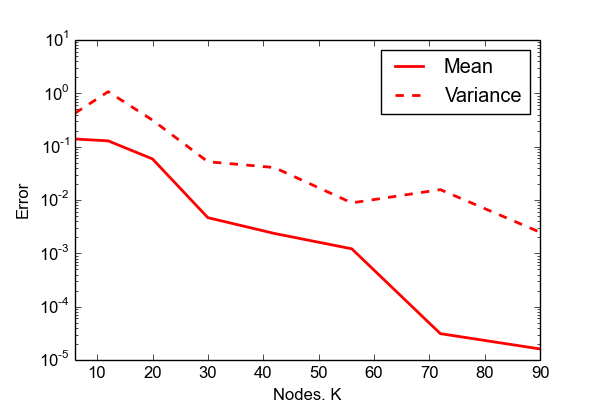
\includegraphics[width = 0.85\textwidth]{convergence_dependence.png}
 \end{figure}
 \end{frame}


 % TODO
 % use contourf
 \begin{frame}
 \frametitle{All random variables can with aid of the Rosenblatt transformations be transformed to/from the uniform distribution}
 \begin{figure}
 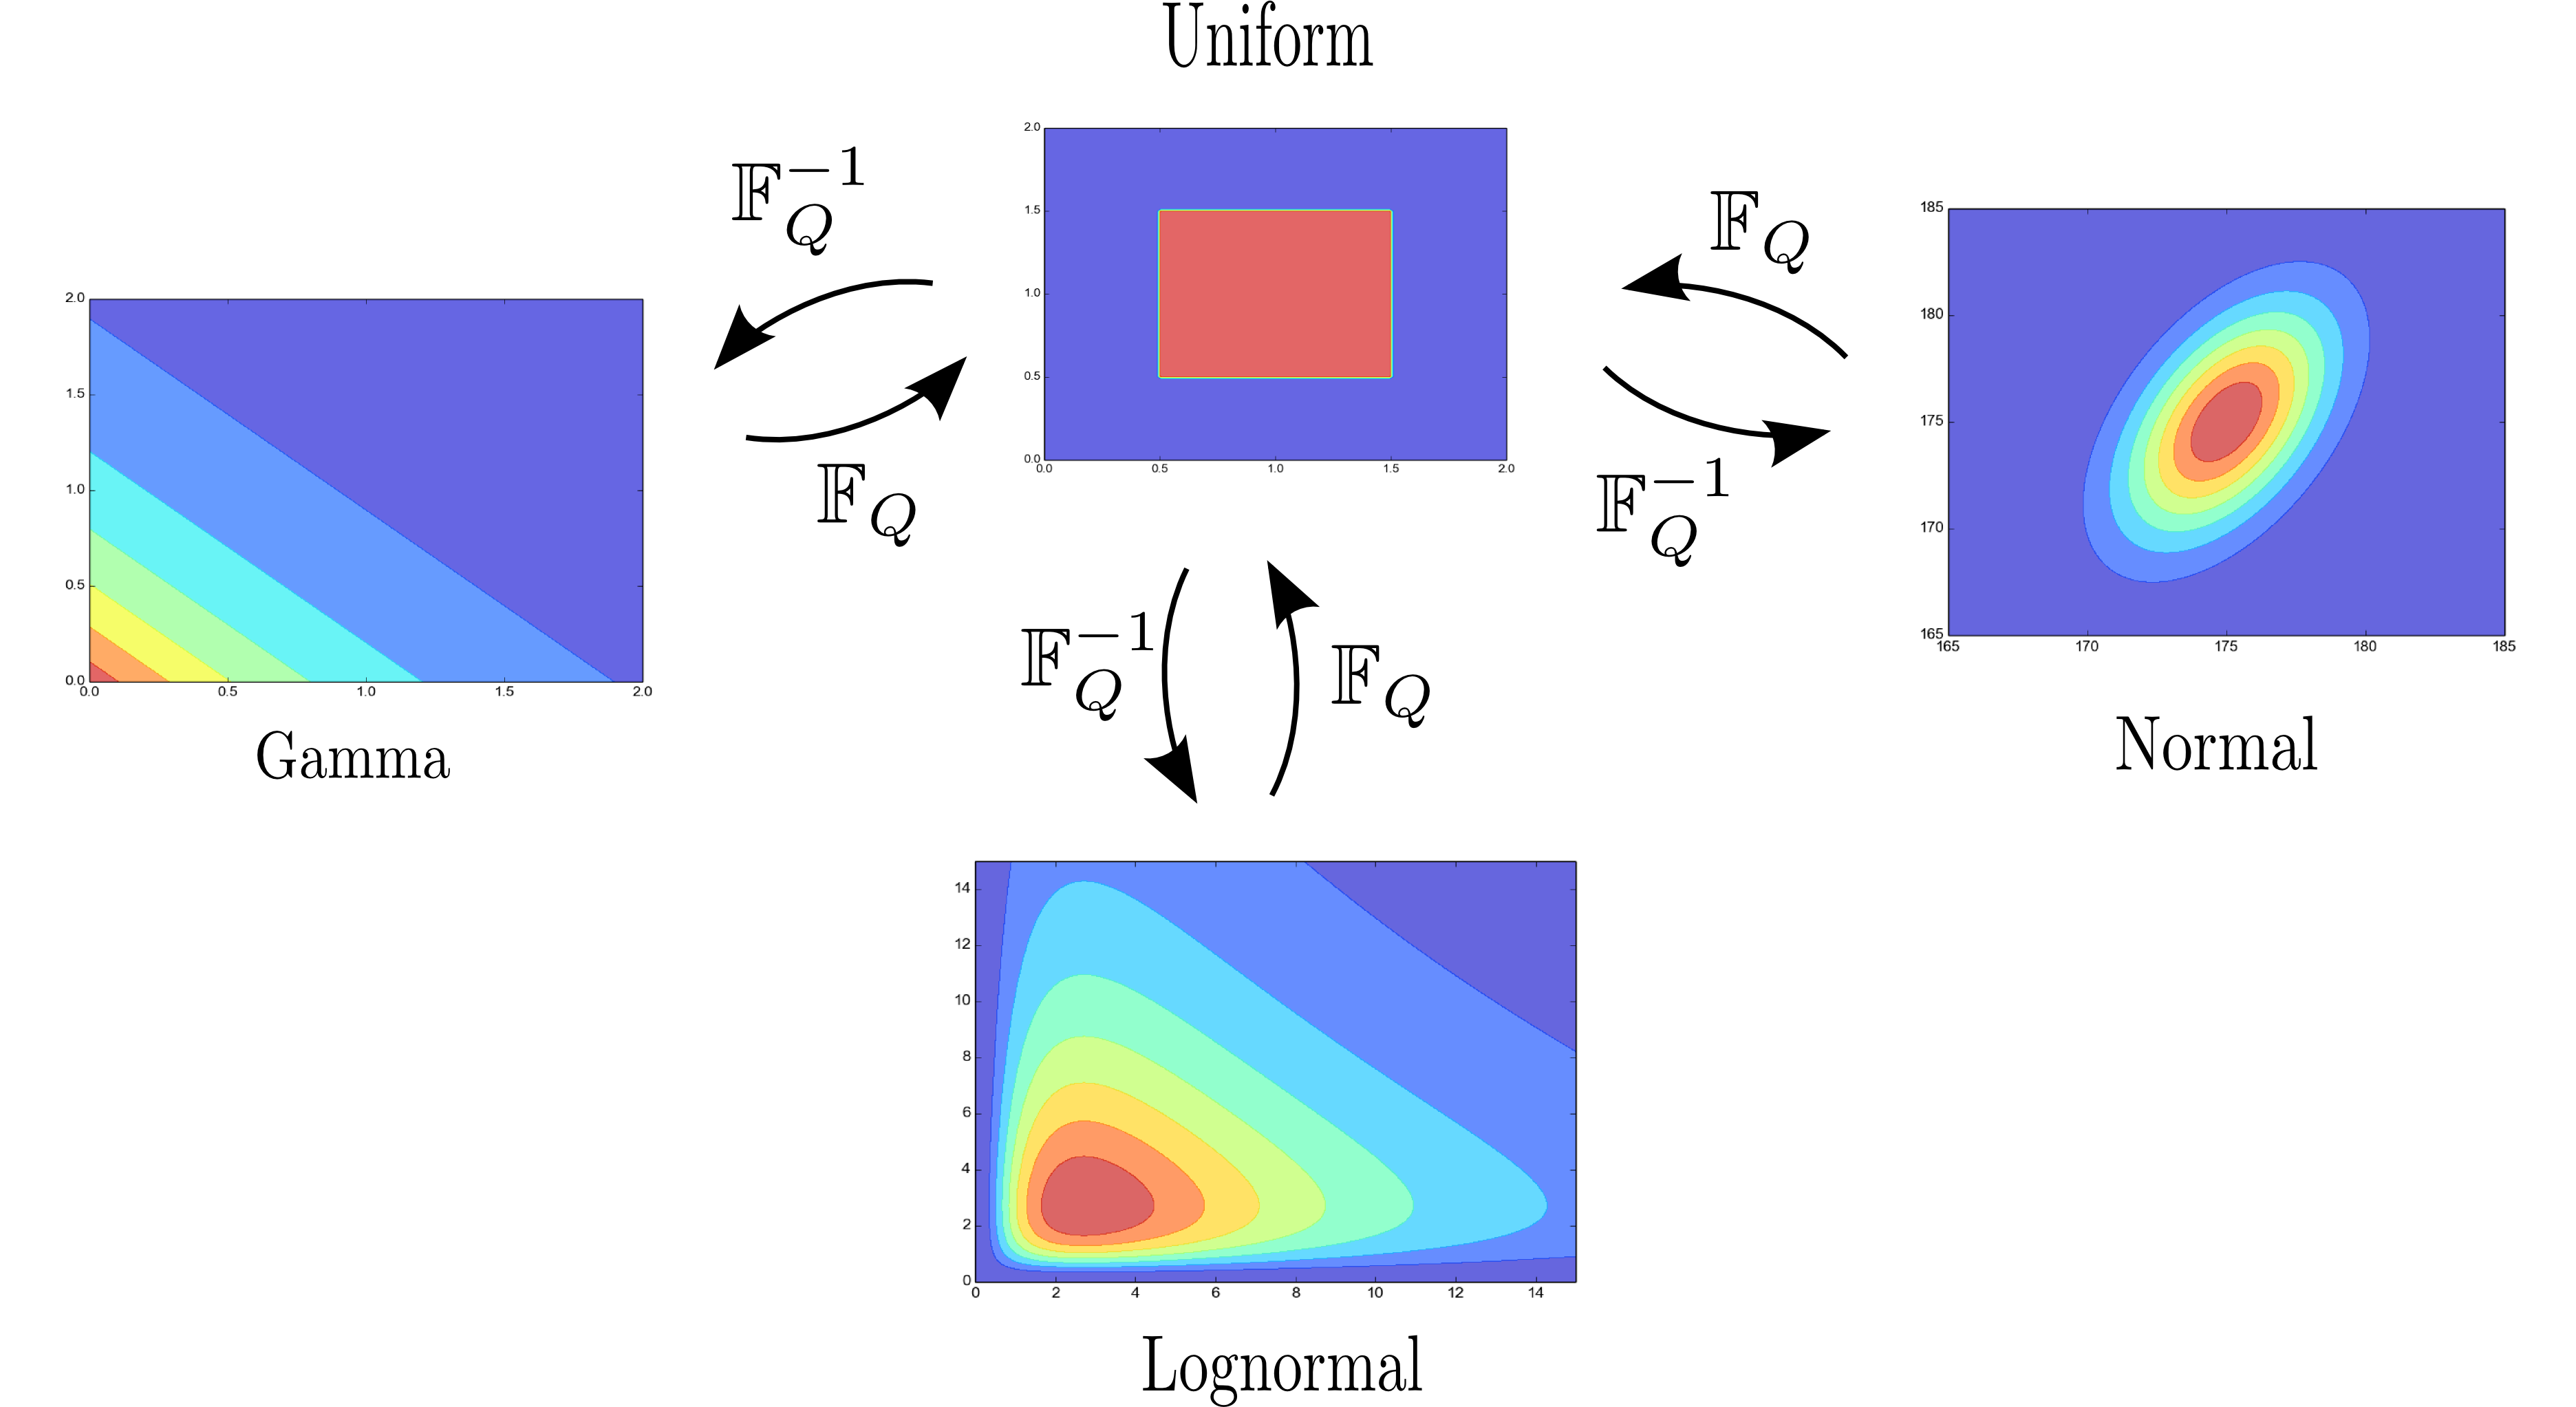
\includegraphics[width = \textwidth]{distributions.png}
 \end{figure}

 \end{frame}

 \begin{chaospy}{Point collocation with Rosenblatt transformation}
 \scriptsize
 \begin{lstlisting}[language=Python]
def u(x,a, I):
    return I*np.exp(-a*x)
|\pause|
dist_R = cp.J(cp.Normal(), cp.Normal())
C = [[1, 0.5], [0.5, 1]]
mu = [0, 0]
dist_Q = cp.MvNormal(mu, C)
|\pause|
P = cp.orth_ttr(M, dist_R)|\pause|
nodes_R = dist_R.sample(2*len(P), "M")|\pause|
nodes_Q = dist_Q.inv(dist_R.fwd(nodes_R))
|\pause|
x = np.linspace(0, 1, 100)
samples_u = [u(x, *node) for node in nodes_Q.T]|\pause|
u_hat = cp.fit_regression(P, nodes_R, samples_u)
\end{lstlisting}
\end{chaospy}

 \begin{frame}
 \frametitle{Convergence of point collocation with Rosenblatt transformations}
 \begin{figure}
 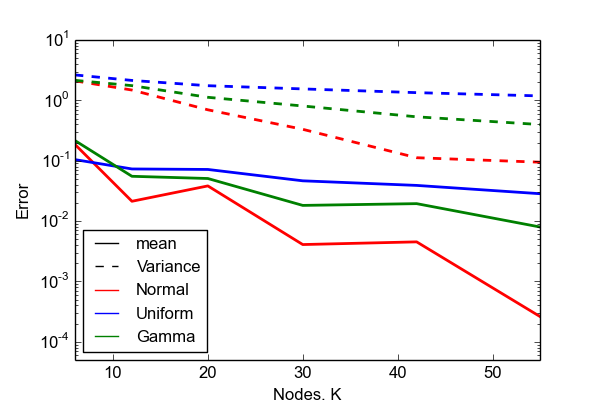
\includegraphics[width = 0.9\textwidth]{rosenblatt2.png}
 \end{figure}
 \end{frame}

 \begin{frame}{Rosenblatt transformations is essentially variable substitution}{}
     \begin{align*}
     \qquad\E{u} = \int u(x; q)& f_Q(q)\,dq &
     \onslide<5->{= \int &u\left(x; q\right)
     f_Q(q) \frac{f_R(r)}{f_Q(q)}\,dr} \qquad\qquad & &\\ \\
     \onslide<2->{F_Q(q) &= F_R(r)} &
     \onslide<4->{q &= F^{-1}_Q\left( F_R(r) \right)} \\
     \onslide<3->{f_Q(q)\,dq &= f_R(r)\,dr} &
     \onslide<4->{dq &= \frac{f_R(r)}{f_Q(q)}\,dr}
     \end{align*}
 \end{frame}

 \begin{chaospy}{Pseudo-spectral with Rosenblatt transformation}
 \scriptsize
 \begin{lstlisting}[language=Python]
def u(x,a, I):
    return I*np.exp(-a*x)
|\pause|
C = [[1,0.5],[0.5,1]]
mu = np.array([0, 0])
dist_R = cp.J(cp.Normal(), cp.Normal())
dist_Q = cp.MvNormal(mu, C)

P = cp.orth_ttr(M, dist_R)
nodes_R, weights_R = cp.generate_quadrature(M+1, dist_R)|\pause|
nodes_Q = dist_Q.inv(dist_R.fwd(nodes_R))|\pause|
weights_Q = weights_R*\
    dist_Q.pdf(nodes_Q)/dist_R.pdf(nodes_R)
|\pause|
x = np.linspace(0, 1, 100)
samples_u = [u(x, *node) for node in nodes_Q.T]|\pause|
u_hat = cp.fit_quadrature(P, nodes_R, weights_Q, samples_u)
\end{lstlisting}
\end{chaospy}

 \begin{frame}
 \frametitle{Convergence of pseudo-spectral projection with Rosenblatt transformations}
 \begin{figure}
     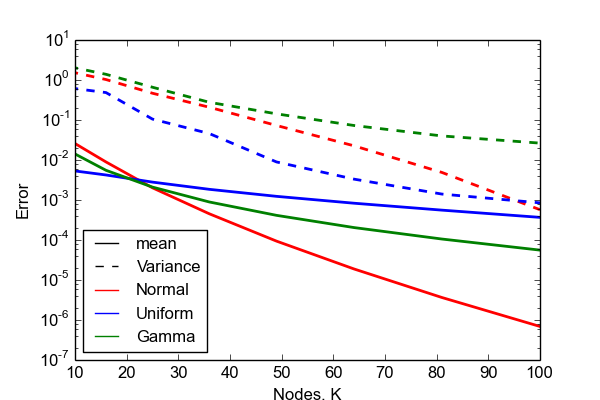
\includegraphics[width = 0.9\textwidth]{rosenblatt.png}
 \end{figure}
 \end{frame}

 
\begin{frame}[fragile]{Thank you}
  \begin{center}
     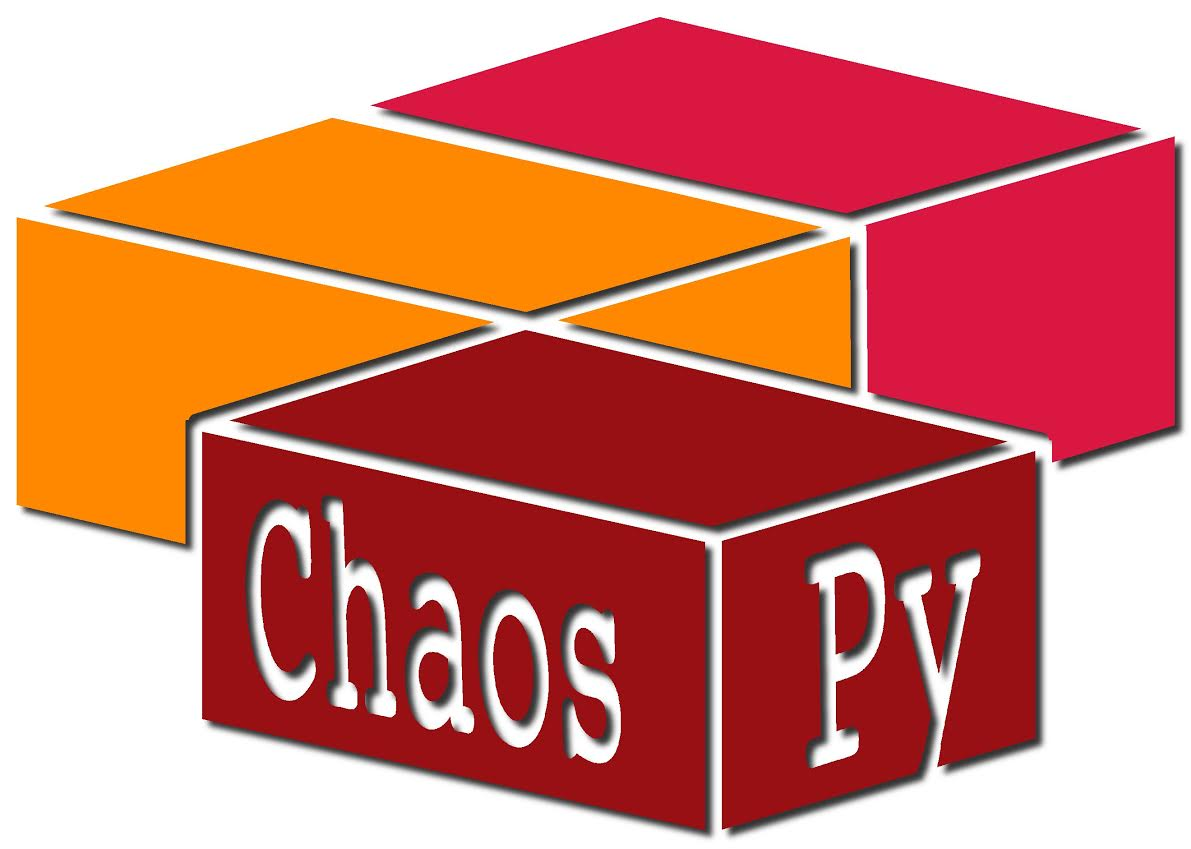
\includegraphics[width=.5\textwidth]{chaospy_logo.jpg}
  \end{center}
    \begin{alert}{A very basic introduction to scientific Python programming:}
    \scriptsize
      \href{http://hplgit.github.io/bumpy/doc/pub/sphinx-basics/index.html}{http://hplgit.github.io/bumpy/doc/pub/sphinx-basics/index.html}\\
%\verb;http://hplgit.github.io/bumpy/doc/pub/sphinx-basics/index.html;
  \end{alert}
  \begin{alert}{Installation instructions:}\\
  \scriptsize
      \href{https://github.com/hplgit/chaospy}{https://github.com/hplgit/chaospy}\\
%\verb;http://github.com/hplgit/chaospy/;
  \end{alert}
%     \begin{alert}{Interactive session:}\\
%   \scriptsize
% \href{http://10.50.3.247:8888/}{http://10.50.3.247:8888/}
% 
% %\verb;http://10.50.3.247:8888/;
%   \end{alert}
\end{frame}


\end{document}
